%*******************************************
\section{Phishing Survey}
%*******************************************
\label{s:prestudy}
Before elaborating on the concrete app design we ran a small phishing survey.
 To the best of our knowledge there do not exist other surveys which resemble ours and additionally were conducted in Germany.
 This chapter deals with the main objectives of the survey.
 Furthermore, it provides some details and finally presents the results and evaluates the questionnaire.


%============================================
\subsection{Main Objectives}
%============================================
Our main objectives of this survey were twofold:

\begin{enumerate}
	\item \textbf{Awareness and Knowledge} One goal of the survey was to comprehend what exactly Internet users understand under phishing.
 With a Likert scale we furthermore tried to figure out how they evaluate their on knowledge on the topic of Internet security.

	\item \textbf{Preferences of Users} Another purpose of the survey was to get an idea of the users' preferences with regard to an educational app.
 For example, they were asked whether they found a quiz based game appropriate for learning purposes.

\end{enumerate}
%============================================
\subsection{Survey Details}
%============================================
This section provides some details about our questionnaire, how we distributed it and how we filtered the surveys in order to consider our target group for the results and evaluation.

The whole survey form can be found in \autoref{s:presurvey_form}.

\subsubsection{Questionnaire}
In the following we present the structure of our questionnaire and the function of each section.
 
\begin{enumerate}
	\item \textbf{General Information} In this section the participant is asked to provide information regarding his gender, age, his professional qualification as well as his field of study or work.
 The main purpose of this section is to exclude participants which do not fit into our target group.

	\item \textbf{Internet Usage} Here, the participant is asked how often he uses the Internet, whether he owns a smartphone and which applications he uses on his desktop computer and which ones he uses on his smartphone.
 This section is intended to give us an overview of the users' Internet usage and helps us to exclude participants who do not fit into our target group.

	\item \textbf{Self-Assessment} In this part of the survey, the participant has to indicate how much he agrees to the presented statements with the aid of a Likert scale.
 The statements mainly refer to their self-assessment regarding their knowledge about Internet security.
 For example, they have to assess, whether they think they have enough knowledge, to avoid the dangers of the Internet or whether they think it is easy for them to distinguish legitimate e-mails from fake ones.
 This section is partially based on Likert scale statements used by DIVSI\cite{divsi2012divsi}.
	\item \textbf{Phishing} Here, the participant gets concrete questions to the topic of phishing.
 In particular, he is asked which services and which user information are endangered by phishing attacks.
 This section purposes to find out what the participants know about and think of phishing.

	\item \textbf{Anti-Phishing App} This section asks the user for his preferences regarding an anti-phishing education app.
 With the aid of a Likert scale he is requested to assess, for example, whether the would like having a game with a fish, or whether he finds a text-based approach meaningful as well as whether he would have fun with a question-answer quiz game.

	\item \textbf{Further Survey Progress} In this part of the survey the user can provide us his e-mail address in case he wants to get information about the further progress of the survey or would like to test the app.

\end{enumerate}

\subsubsection{Distribution}
In total 251 persons participated in our survey.
 We set up an online survey as well as asked students to fill out our printed survey.
 In the following we briefly explain our distribution process.


\begin{description}[leftmargin=0cm]
	\item[Printed Survey] To reach participants for our printed survey we contacted multiple professors and asked them whether we could have 10 minutes of their lecture time to have their students fill out our printed survey.
 Moreover, we asked our friends and parents whether they can ask their friends, colleague or customers to fill out the questionnaire.

	\item[Online Survey] The online survey was mainly distributed digitally.
 We contacted our friends and asked them to participate in the survey.
 We also demanded to forward the link to their friends so we could reach a wider range of people.

\end{description}

\subsubsection{Filtering for Evaluation}

\autoref{table:prestudy_filter} summarizes what kind of answers we used in order to exclude participants from the survey who do not fit into our target group.
\begin{table}[hHtbp]
\centering
    \begin{tabular}{ | p{5cm} | p{10cm} |}
    \hline\textbf{Question} & \textbf{Filtering}  \\  \hline
		\hline\  Age & We consider all adults ranging from 18 - 65 years.
 \\
    \hline\  Gender & We do not exclude any gender.
 \\ 
    \hline\  Professional qualification & The participant does not have to exhibit a specific professional qualification to be considered for the results and evaluation.
 \\ 
		\hline\  Field of study/work & Students, employees or employers in the field of computer science or electrical engineering are filtered out as they do not belong to our target group.
 \\ 
	  \hline\ Frequency of Internet usage & Participants who have indicated ``rarely'' as the answer to this question do not belong to our target group and thus are filtered out.
 \\ 
	  \hline\ Used Internet applications  &  The listed applications include, for example, browser, e-mail, shopping as well as banking.
 Any service of the Internet is potentially endangered by phishing.
 For this reason we do not use this question to filter out participants.
\\ 
    \hline\ Owning a smartphone  & With the app we particularly target smartphoner owners.
 For this reason participants who do not own any kind of smartphone are filtered out.
 \\
		\hline\ Used smartphone applications in the Internet  & The listed applications include, for example, browser, e-mail, shopping as well as banking.
 Any service of the Internet, especially on a smartphone, is potentially endangered by phishing.
 For this reason we do not use this question to filter out participants.
 \\
    \hline\ Number of received commercial e-mails per week  & We do not filter out any participant with this question.
 \\
    \hline\ Number of received e-mails asking for personal data  & We do not filter out any participant with this question.
 \\
    \hline\ User reads up on topics related to dangers in the Internet  &  Participants who have chosen ``no'' as answer are filtered out.
 We specifically target users who are interested in getting safer in the Internet.
 As the participants who have indicated ``no'' do not seem to have any interest in doing so, they will most likely do not show interest in our app.
 For this reason we regard them as not belonging to our target group and exclude them from the analysis and evaluation.
\\
    \hline\  Section to self-assessment regaring their knowledge about Internet security &  We do not filter out any participant with these statements.
\\
		\hline\  Section to questions concretely related to phishing & We do not filter out any participant with these statements.
 \\
    \hline\  Section to preferences for an anti-phishing education app & We do not filter out any participant with these statements.
\\
    \hline
    \end{tabular}
    \caption{Filtering rules for the phishing survey}
    \label{table:prestudy_filter}
    
\end{table}

In the succeeding section we present and evaluate the results of the study.
 With the filtering above we had 169 remaining participants who were considered for the evaluation.

%============================================
\subsection{Results and Evaluation}
%============================================
The study yielded interesting results which should be considered when designing an anti-phishing education app, either for this work, or if not possible due to time constraints in future work.
 This section outlines the results of the study.


\begin{description}[leftmargin=0cm]
	\item[General Information] The ratio of our male and female survey participants was more or less balanced.
 40.83\% of the users were female and 56.80\% of them were male.
 The remaining 2.37\% did not indicate any gender.
 The average age of our participants is 27.59, the youngest participants are 19 years old, the oldest are 63 years old.
 Most of the survey participators, 48.52\%, obtained a university degree.
 24.85\% of them do not have any professional qualification (yet). 17.75\% did an apprenticeship and the remaining participants had a master craftsman certificate or did not indicate any professional qualification in the survey.
	
	\item[High Rate of Android Users] The majority of the participants were Android users.
 In total about 60\% of the study participants use an Android smartphone.
 The remaining 40\% are iOS users.
 This result roughly relates to the general market share for these platforms and additionally supports our decision for the implementation of an Android application.

	\item[High Internet Usage Frequency] 51.48\% of the users are online several times a day.
 Another 30.18\% indicated that they are online even constantly.
 As a consequence, over 80\% of the survey participants are frequently online.
 This is depicted in \autoref{fig:internet_usage} Being online is always connected with being attackable and vulnerable to dangers of the Internet, such as phishing attacks, while the extent of the vulnerability of course depends on the expertise of the person being online.
 However, the more often a user is in the Internet, the more likely it is that he will experience a phishing attempt.

	
	\item[Usage Distribution of Internet Applications] \autoref{fig:desktop_apps}~and~\autoref{fig:smartphone_apps} summarize the usage distribution of Internet applications on a desktop computer and on smartphones.
 Almost all participants, 99.41\%, make use of e-mails on their desktop computer.
 88.76\% of the smartphone owners use their e-mail application on the smartphone, which is still a high percentage.
 As we have previously mentioned, cf. \autoref{s:attack_channels}, e-mail is a common attack channel for phishing attempts.
 Consequently, all users of e-mail applications as well as users of webmail on mobile phones are potentially endangered by phishing attacks.
 The same applies to participants using browsers.
 A common way to trick users to disclose their confidential information is the use of fake websites.
 These websites can be reached by clicking on a link in an e-mail, SMS, in online social networks or instant messaging systems as well as by simply surfing in the Internet.
 About 80\% of all considered participants make use of desktop or smartphone browsers.
 Furthermore, it is conspicuous that banking is far less used on the smartphones compared to desktop computers.
 While about 74.56\% of the participants make use of online banking on the desktop computer, only 26.63\% make use of it on their smartphones, which is however still a quarter of the participants.
	The question to ask here is if these users use the browser for the online banking or if they use apps provided by their bank.
 Regardless of the answer to this question, these users might be more likely to react to phishing e-mails, claiming to come from their bank, on their smartphone compared to other users who manage their financial arrangements on a desktop computer and thus are less likely to access a phishing website, cf. \autoref{s:antiphishing_on_smartphone}. To sum it up, all the categories of applications are used by the participants, on their smartphones as well as on their desktop computers.
 For this reason, all of these application categories should be reflected in the choice of the example URLs for the final app.
 For future work, one could argue to put the focus on URLs from specific categories (also those which were not considered for the study), depending on the usage distribution.


	\item[Self-Assessment - Knowledge to avoid dangers of Internet] 18.34\% of the participants think, that they have enough knowledge to avoid the dangers of the internet.
 Further 45.56\% agree with the statement and only about 13\% disagree or strongly disagree with this statement.
 As a consequence the majority of the participants were quite confident that they could avoid the security-related risks raised by the Internet.
 
	
	\item[Self-Assessment - Distinguish legitimate from illegitimate e-mails] 87.23\% of the participators think that they can easily distinguish legitimate e-mails from fake onesstrongly.
 Only about 8\% of the participant did not agree or strongly disagreed with this statement.
 This arouses the suspicion that the users are not aware of how easy it is to spoof the ``from'' field of an e-mail or to create credible message contents which in fact may persuade the receiver to be trustful.

	
	\item[Self-Assessment - Trust to e-mails from known parties] The majority of the participants trust e-mails which come from persons they know.
 Approximately 20\% strongly agreed and approximately 57\% agreed with this statement.
 Only about 2\% strongly disagreed and approximately 5\% of the participants disagreed with this statement.
 This again shows, that most of the participants are not aware that spoofing the ``from field'' of an e-mail is very easy.
 These users are likely to react to e-mails which claim to be, for example, from friends.
 Such e-mails may contain links to the download of malware or malicious websites.


	\item[Self-Assessment - Internet security is only related to financial applications] With a Likert scale the participants had to indicate how much they agreed with the following statement: ``Internet security is only related to financial applications''. The answers to this statement showed that the majority of the participants are aware that security related issues in the Internet do not solely concern financial applications.
 49.7\% of the users strongly disagreed with this statement and another 24.26\% disagreed.
 Only about 10\% of the participators agreed or strongly agreed with this statement and about 14\% indicated ``neither nor'' as an answer.
 Even though most users seem to be aware that Internet risks do not only concern financial applications, the ones who are not aware that, phishing for example, can also occur in online social networks, should be enlightened about this.
 To do this, originally, our plan was to display the consequences of falling for a certain phishing website (phishing URL). In this way, the user could have learnt what his loss could have been, if he had fallen for such an attack in reality.
 This would have contributed to his awareness that security issues in the Internet, in this particular case phishing, are not necessarily related to financial loss only.
 Due to lack of time we could not realize this approach, so it is something which should be considered in future work.


	\item[Services endangered by phishing] \autoref{fig:endangered_services} summarizes the results for this question.
 All in all, we can observe that the participants agree that phishing can actually occur related to any service.
 The users agree (97.04\%) that especially the e-mail service is endangered by phishing.
 Also they see the browser with fake websites (70.41\%), online banking (83.43\%) as well as social networks (74.56\%) as endangered.
 Still about 40\% consider various media (audio and video) services as well as online games as endangered.
 These services are in fact not targeted as often as other services in the Internet, however they are potential targets and should be communicated to the user, for example, with the aid of the choice of the URLs to decide on.

	\item[Data endangered by phishing] \autoref{fig:endangered_data} outlines the results of this question and illustrates that the participants agree that any kind of data is potentially endangered by phishing attacks.
 90.53\% of the participants are of the opinion that login data is endangered by phishing.
 About 89\% agree that credit card information as well as personal data is endangered, too.
 Finally, 76.33\% of the participants consider PINs and TANs endangered.
 Consequently, there does not seem to be a major necessity in enlightening users in this area.

	\item[Preferences for an education app] This section influenced how our app is designed. There were three results that we took into consideration.
	First, most of the users (50.8\%) stated clearly against an app that uses a fish as the main character. 
	Second, most of the users either voted for a quiz based game (51.5\%) or did not care (33.1\%).
	The minority of the participants voted against a quiz based game (13\%).
	Finally, users were quite neutral regarding text based learning programs (40.8\%).
	For these reasons, we could confirm our desired approach of a quiz based game, with introductory parts that also contain text, cf. \autoref{s:approach}.
	The other results from this section remain to be considered for future work.
	These include aspects, such as dividing the program into exercise and test mode.
	%\item[VERGLEICHE?]
\end{description}


\begin{figure}[hHtbp]
\centering
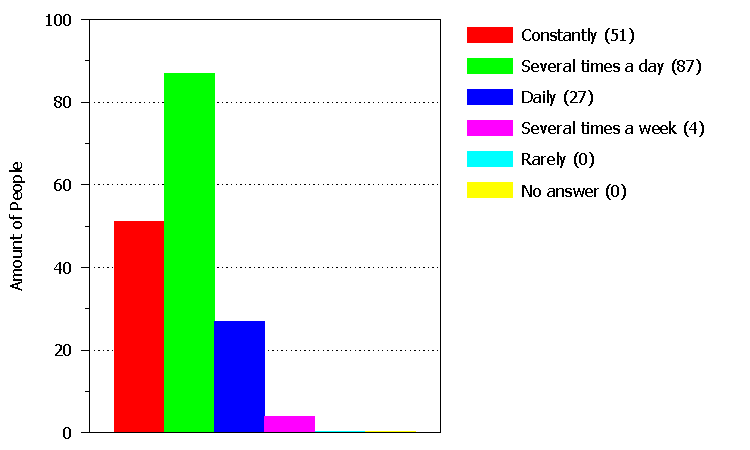
\includegraphics[width=1.0\textwidth]{201_Frequency_of_Internet_Usage.pdf}
\caption{Frequency of Internet Usage}
\label{fig:internet_usage}
\end{figure}


\begin{figure}[hHtbp]
\centering
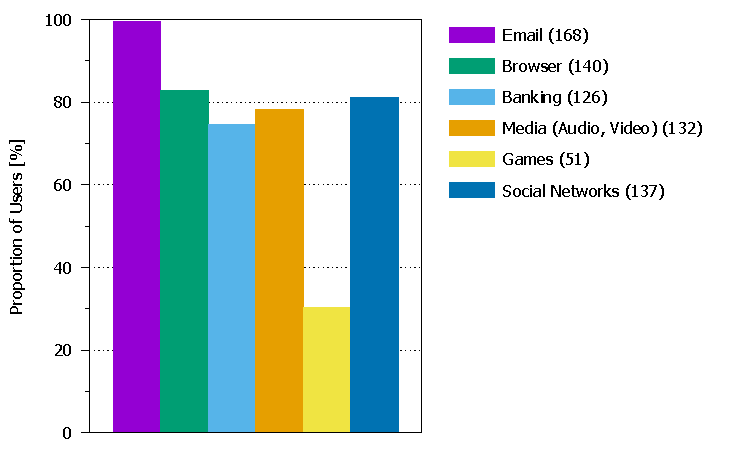
\includegraphics[width=1.0\textwidth]{202_Usage_Applications_Desktop.pdf}%
\caption{Usage of Internet Applications on Desktop Computers}%
\label{fig:desktop_apps}%
\end{figure}

\begin{figure}[hHtbp]
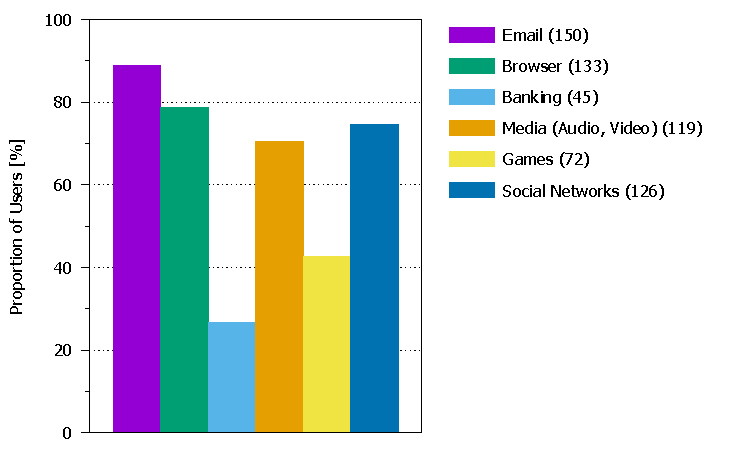
\includegraphics[width=1.0\textwidth]{204_Usage_Applications_Smartphone.pdf}%
\caption{Usage of Internet Applications on Smartphones}%
\label{fig:smartphone_apps}%
\end{figure}

\begin{figure}[hHtbp]
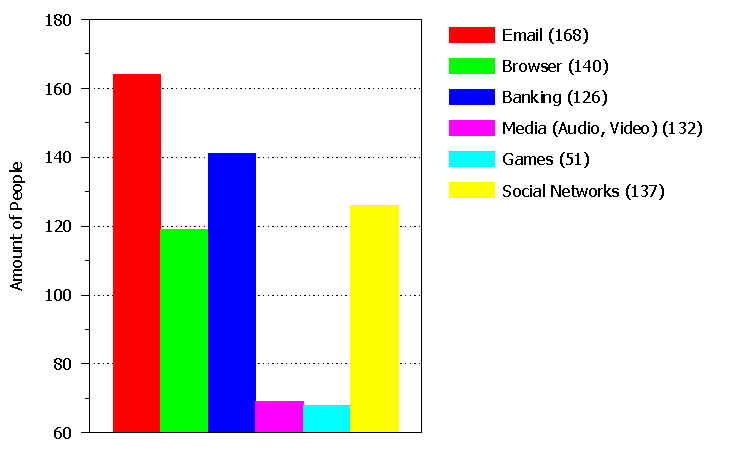
\includegraphics[width=1.0\textwidth]{401_Endangered_Services.pdf}%
\caption{Services Endangered By Phishing}%
\label{fig:endangered_services}%
\end{figure}

\begin{figure}[hHtbp]
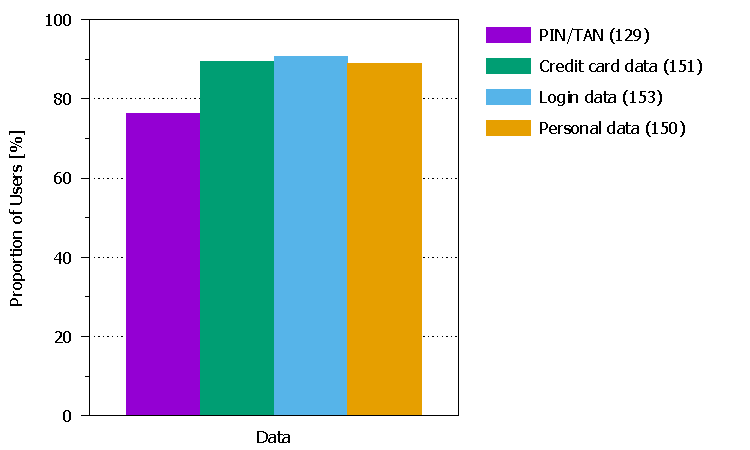
\includegraphics[width=1.0\textwidth]{402_Endangered_Data.pdf}%
\caption{Data Endangered By Phishing}%
\label{fig:endangered_data}%
\end{figure}
